\documentclass{article}

\usepackage[table]{xcolor}
\usepackage{fancyhdr}
\usepackage{graphicx}
\graphicspath{ {images/} }
\usepackage{extramarks}
\usepackage{amsmath}
\usepackage{amsthm}
\usepackage{amsfonts}
\usepackage{tikz}
\usepackage[plain]{algorithm}
\usepackage{algpseudocode}
\usepackage{bbm}

\usetikzlibrary{automata,positioning}

%
% Basic Document Settings
%

\topmargin=-0.45in
\evensidemargin=0in
\oddsidemargin=0in
\textwidth=6.5in
\textheight=9.0in
\headsep=0.25in

\linespread{1.1}

\pagestyle{fancy}
\lhead{\hmwkAuthorName}
\chead{\hmwkTitle}
\rhead{\firstxmark}
\lfoot{\lastxmark}
\cfoot{\thepage}

\renewcommand\headrulewidth{0.4pt}
\renewcommand\footrulewidth{0.4pt}

\setlength\parindent{0pt}

%
% Create Exercise Sections
%

\newcommand{\enterExerciseHeader}[1]{
    \nobreak\extramarks{}{Question \arabic{#1} continued on next page\ldots}\nobreak{}
    \nobreak\extramarks{Question \arabic{#1} (continued)}{Question \arabic{#1} continued on next page\ldots}\nobreak{}
}

\newcommand{\exitExerciseHeader}[1]{
    \nobreak\extramarks{Question \arabic{#1} (continued)}{Question \arabic{#1} continued on next page\ldots}\nobreak{}
    \stepcounter{#1}
    \nobreak\extramarks{Question \arabic{#1}}{}\nobreak{}
}

\setcounter{secnumdepth}{0}
\newcounter{partCounter}
\newcounter{homeworkExerciseCounter}
\setcounter{homeworkExerciseCounter}{1}
\nobreak\extramarks{Question \arabic{homeworkExerciseCounter}}{}\nobreak{}

\newenvironment{homeworkExercise}{
    \section{Question \arabic{homeworkExerciseCounter}}
    \setcounter{partCounter}{1}
    \enterExerciseHeader{homeworkExerciseCounter}
}{
    \exitExerciseHeader{homeworkExerciseCounter}
}

%
% Homework Details
%   - Title
%   - Due date
%   - Class
%   - Section/Time
%   - Instructor
%   - Author
%

\newcommand{\hmwkTitle}{Mini Project}
\newcommand{\hmwkDueDate}{December 3, 2017}
\newcommand{\hmwkClass}{Introduction to Graphical Models}
\newcommand{\hmwkClassTime}{}
\newcommand{\hmwkClassInstructor}{Taught by Assisitant Professor Umut Simsekli}
\newcommand{\hmwkAuthorName}{Pengfei MI, Rui SONG, Yanting LI}

%
% Title Page
%

\title{
    \vspace{2in}
    \textmd{\textbf{\hmwkClass:\ \hmwkTitle}}\\
    \normalsize\vspace{0.1in}\small{Due\ on\ \hmwkDueDate\ at 11:55 pm}\\
    \vspace{0.1in}\large{\textit{\hmwkClassInstructor\ \hmwkClassTime}}
    \vspace{3in}
}

\author{\textbf{\hmwkAuthorName}}
\date{}

\renewcommand{\part}[1]{\textbf{\large Part \Alph{partCounter}}\stepcounter{partCounter}\\}

%
% Various Helper Commands
%

% Useful for algorithms
\newcommand{\alg}[1]{\textsc{\bfseries \footnotesize #1}}

% For derivatives
\newcommand{\deriv}[1]{\frac{\mathrm{d}}{\mathrm{d}x} (#1)}

% For partial derivatives
\newcommand{\pderiv}[2]{\frac{\partial}{\partial #1} (#2)}

% Integral dx
\newcommand{\dx}{\mathrm{d}x}

% Alias for the Solution section header
\newcommand{\solution}{\textbf{\large Solution}}

% Probability commands: Expectation, Variance, Covariance, Bias
\newcommand{\E}{\mathrm{E}}
\newcommand{\Var}{\mathrm{Var}}
\newcommand{\Cov}{\mathrm{Cov}}
\newcommand{\Bias}{\mathrm{Bias}}

\begin{document}

\maketitle

\pagebreak


\textit{This document is the report for the Mini-Project of the course "Introduction to Graphical Models" of Master 2 Data Science. 
This project is done in group of three, with group members: Pengfei MI, Rui SONG, and Yanting LI.}


\begin{homeworkExercise}
    Directed graphical model
    \\
    
    \textbf{Solutions:} \\
    The directed graphical model for our model can be drawn like below
    \begin{figure}[h]
    	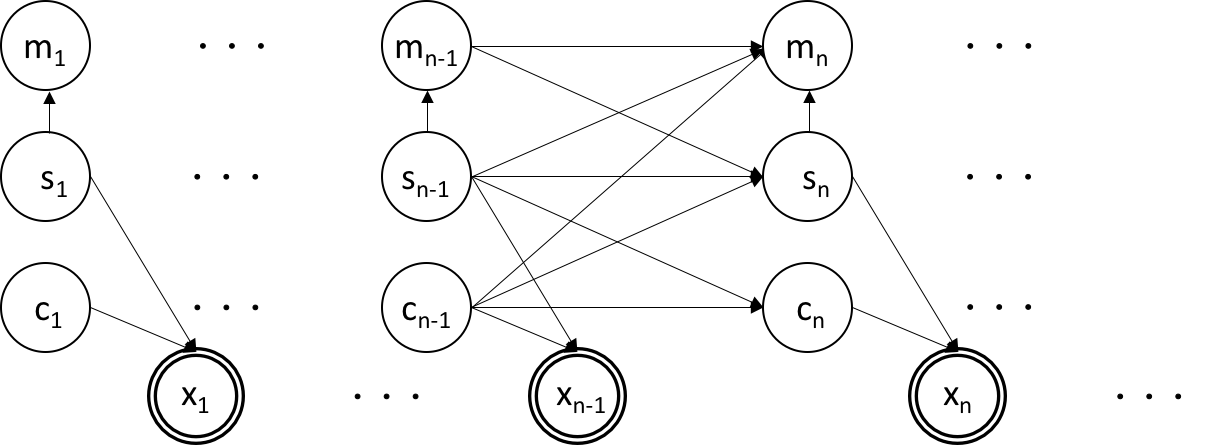
\includegraphics[width = 9cm]{Q1}
	\centering
    \end{figure}

\end{homeworkExercise}

\pagebreak

\begin{homeworkExercise}
	Transition Matrix
	\\
	
	\textbf{Solutions:} \\
	Define a variable $\Psi_{n} \equiv [s_{n}, m_{n}, c_{n}]$. The set of all states can be listed in a vector $\Omega$ then the state of the system at pixel $n$ can be represented as $\Psi_{n} = \Omega(j)$ where $j \in \{1, 2, ..., (S\times M\times C)\}$ and $C = max_{s,k}\mathit{l}(s) $ ($=7$ in our model). Then the transition matrix is:
	\begin{equation}
    	\begin{split}
	A(i, j) &= p(\Psi_{n+1} = \Omega(i) | \Psi_{n} = \Omega(j)) \\
	& = p(c_{n+1} = c_{i}, s_{n+1} = s_{i},  m_{n+1} = m_{i} | c_{n} = c_{j}, s_{n} = s_{j},  m_{n} = m_{j}) \\
	& = p(c_{n+1} = c_{i} | c_{n} = c_{j}, s_{n} = s_{j})p(s_{n+1} = s_{i},  m_{n+1} = m_{i} | c_{n} = c_{j}, s_{n} = s_{j},  m_{n} = m_{j}) \\
	& = p(c_{n+1} = c_{i} | c_{n} = c_{j}, s_{n} = s_{j}) p(s_{n+1} = s_{i} | c_{n} = c_{j}, s_{n} = s_{j}, m_{n} = m_{j}) p(m_{n+1} = m_{i} |s_{n+1} = s_{i}, c_{n} = c_{j}, s_{n} = s_{j})\\
	& = \begin{cases}
			\delta(c_{n+1} - c_{n} -1) \delta(s_{n+1} - s_{n}) \delta(m_{n+1} - m_{n}) &\mbox{if $c_{n} \neq \mathit{l}(s_{n})$}\\
			\delta(c_{n+1} -1)\tau(s_{n+1}|s_{n}, m_{n} )\tau(m_{n+1}|s_{n+1}, m_{n}) &\mbox{if $c_{n} = \mathit{l}(s_{n})$}
	       \end{cases}
	\end{split}
     \end{equation}
     where $\tau(s_{n+1}|s_{n}, m_{n} )$ and $\tau(m_{n+1}|s_{n+1}, m_{n})$ are defined in the description.\\
     Then the observation model can be written like: 
     $$p(x_{n} | \Psi_{n}) = \prod_{i=0}^{1} \mathcal{N}(x_{n}; \mu_{i}, \sigma_{i}^{2}) ^{\mathbbm{1}(f(\Psi_{n})=i)}$$
     
     Then the graphical model becomes:
     \begin{figure}[h]
    	   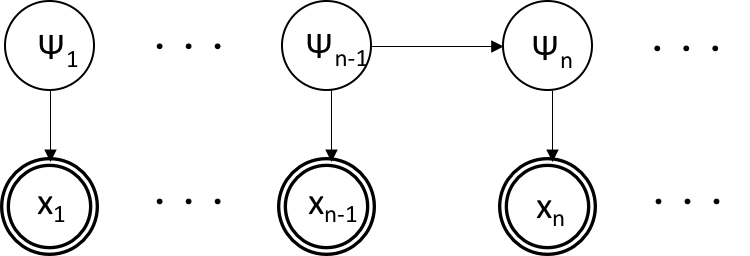
\includegraphics[width = 9cm]{Q2}
	   \centering
     \end{figure}
	
\end{homeworkExercise}

\pagebreak

\begin{homeworkExercise}
	Simulation of HMM
	\\
	
	\textbf{Solutions:} \\
	The general idea to simulate the HMM model is: for each states $j \in \{1,2, ... , (S\times M\times C)\}$, we generate a random number $r$ according to a uniform distribution in the interval $[0, 1]$. Then we find the state $k$ such that $\sum_{i=1}^{k}A(i,j) < r$ and $\sum_{i=1}^{k+1}A(i,j) >= r$. Then we will transfer from state $j$ to state $i$. \\
	For the code, please look at file $template_code.ipynb$. The barcode simulated is :
	\begin{figure}[h]
    		
\includegraphics[width = 9cm]{Q3}
		\centering
         \end{figure}
         As we can see this looks very much like a real scanline. And the barcode string is "184525950079".
	
\end{homeworkExercise}

\pagebreak

\begin{homeworkExercise}
	Fill code part 1, 2, and 3
	\\
	
	\textbf{Solutions:} \\
	Please refer to file "template$\_$code.ipynb".
\end{homeworkExercise}


\begin{homeworkExercise}
	Compute the filtering distribution and marginals
	\\
	
	\textbf{Solutions:} \\
	Please refer to file "Part4.py".
\end{homeworkExercise}

\begin{homeworkExercise}
	Compute the smoothing distribution and marginals
	\\
	
	\textbf{Solutions:} \\
	Please refer to file "Part5.py".
\end{homeworkExercise}

\pagebreak

\begin{homeworkExercise}
	Viterbi algorithm
	\\
	
	\textbf{Solutions:} \\
\end{homeworkExercise}

\pagebreak

\begin{homeworkExercise}
	Ran algorithms on different random barcodes
	\\
	
	\textbf{Solutions:} \\
\end{homeworkExercise}


\end{document}
